\documentclass[10.5pt]{article}
\usepackage[UTF8]{ctex}
\usepackage{amsfonts,amssymb,amsmath,mathtools,geometry,tikz,booktabs,graphicx,float}
\usepackage[fontsize=10.5pt]{fontsize}
\geometry{a4paper,scale=0.7}

\title{\textbf{\Large 多维正方体电阻网络体对角线之间的等效电阻}}
\author{2024届励志AQ班\quad 程昊一}
\date{}

\begin{document}
\vspace*{\fill}
\begin{center}
	\textbf{\huge 多维正方体电阻网络\\[0.5em]体对角线之间的等效电阻}\\[2em]
	{\large 2024届励志AQ班\quad 程昊一}
\end{center}
\vspace{\fill+10cm}
\newpage
\hspace*{-2em}{\Large \textbf{关于作者}}\\[-0.3cm]
\par 程昊一,男,2009年生于洛阳,现(2022年)就读于西安市铁一中学分校,擅长数学与物理,参加数学竞赛,对此有浓厚的兴趣,并且擅长编程算法.
\newpage
\maketitle
\hspace*{-2em}\textbf{[摘要]}\quad 在学习了正方形和正方体电阻网络之间的等效电阻之后,一般的$n$维的情况是什么样子的?正方形或正方体是二维或三维的情况,那我们可以尝试把结果推广到$n$维的情况.这篇文章,我们利用“等势法”化简电路,然后利用代数与集合的语言描述$\mathbb{R}^n$,利用组合数学计算每一类边的数量,从而解决问题.\\
\textbf{[关键词]}\quad 多维正方体\quad 等效电阻\quad 电阻网络\quad $\mathbb{R}^n$
\section{电阻的基本知识}
由[1]与[2],我们可以得知以下基本知识:
\subsection{电阻的串并联}\label{sec:chuanbing}
若$A,B$之间串联了$n$个电阻,阻值分别为$R_1,R_2,\cdots,R_n$,那么$AB$之间的等效电阻$R$满足下列关系式:
\begin{equation}\label{equ:chuanlian}
R=\sum\limits_{i=1}^{n}R_i.
\end{equation}
\par 若$A,B$之间并联了$n$个电阻,阻值分别为$R_1,R_2,\cdots,R_n$,那么$AB$之间的等效电阻$R$满足下列关系式:
\begin{equation}\label{equ:binglian}
\frac{1}{R}=\sum\limits_{i=1}^{n}\frac{1}{R_i}.
\end{equation}
特别地,若$R_1=R_2=\cdots=R_n=R_0$,那么
\begin{equation}\label{equ:binglian2}
R=\frac{1}{n}R_0.
\end{equation}
\begin{figure}[H] %电阻的串并联图
	\centering
	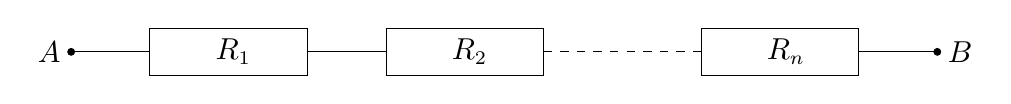
\begin{tikzpicture}
		\fill (0,0)node[left]{$A$} circle(0.05);
		\draw (0,0)--(1,0);
		\foreach \x in{1,4,8}
			\draw (\x,-0.3)rectangle(\x+2,0.3);		
		\draw (3,0)--(4,0);
		\draw [dashed](6,0)--(8,0);
		\draw (10,0)--(11,0);
		\fill (11,0)node[right]{$B$} circle(0.05);
		\node at(1.7,0)[right]{$R_{1}$};
		\node at(4.7,0)[right]{$R_{2}$};
		\node at(8.7,0)[right]{$R_{n}$};
	\end{tikzpicture}
	\caption{电阻的串联}\vspace{1cm}
	\label{fig:chuanlian}
	
	\begin{tikzpicture}
		\fill (0,0)node[left]{$A$} circle(0.05);
		\fill (1,0) circle(0.03);
		\draw (0,0)--(1,0);
		\draw (1,1.5)--(1,-1.5);
		\foreach \y in{1.5,0.5,-1.5}{
			\draw (1,\y)--(2,\y);
			\draw (2,{\y-0.3})rectangle(4,{\y+0.3});
			\draw (4,\y)--(5,\y);
			\fill (1,\y) circle(0.03);
			\fill (5,\y) circle(0.03);
		}
		\draw (5,1.5)--(5,-1.5);
		\draw (5,0)--(6,0);
		\fill (5,0) circle(0.03);
		\fill (6,0)node[right]{$B$} circle(0.05);
		\node at(2.7,1.5)[right]{$R_1$};
		\node at(2.7,0.5)[right]{$R_2$};
		\node at(2.85,-0.5)[right]{$\vdots$};
		\node at(2.7,-1.5)[right]{$R_n$};
	\end{tikzpicture}
	\caption{电阻的并联}
	\label{fig:binglian}
\end{figure}
\subsection{等势法}
我们发现,在电路中,有些点是对称的,它们的地位(电势)是完全相同的,那么我们可以在它们之间任意连接导线或电阻,也可以将它们之间的导线或电阻拆除.例如在图\ref{fig:dengshi}中,$A$与$B$是等势的,所以我们可以将$AB$之间的电阻拆除,从而化简电路.

\begin{figure}[htbp]%等势法图
\centering

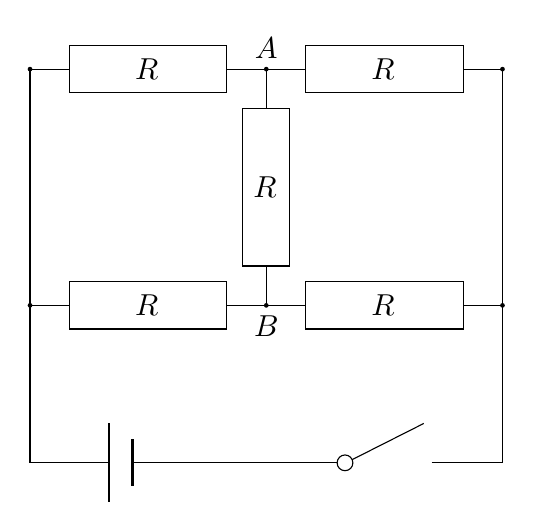
\begin{tikzpicture}
	\draw (0,0)--(1,0);
	\draw [thick](1,0.5)--(1,-0.5);
	\draw [thick](1.3,0.3)--(1.3,-0.3);
	\draw (1.3,0)--(3.9,0);
	\draw (4,0) circle(0.1);
	\draw (4.09,0.04)--(5,0.5);
	\draw (5.1,0)--(6,0);
	\draw (0,0)--(0,5);
	\foreach \x in {0,2.5,3,5.5}{
		\foreach \y in{2,5}
			\draw (\x,\y)--(\x+0.5,\y);
	}
	\foreach \x in {0,3,6}{
		\foreach \y in {2,5}
			\fill (\x,\y) circle(0.03);
	}
	\draw (6,5)--(6,0);
	\draw (3,2)--(3,2.5);
	\draw (3,4.5)--(3,5);
	\draw (2.7,2.5) rectangle(3.3,4.5);
	\node at(2.7,3.5)[right]{$R$};
	\foreach \x in{0.5,3.5}{
		\foreach \y in {1.7,4.7}{
			\draw (\x,\y) rectangle(\x+2,\y+0.6);
			\node at(\x+0.7,\y+0.3)[right]{$R$};
		}		
	}
	\node at(3,2)[below]{$B$};
	\node at(3,5)[above]{$A$};
\end{tikzpicture}
\caption{等势法}
\label{fig:dengshi}
\end{figure}
\section{一维、二维与三维的情况}
一维的情况很简单,就是一根阻值为$R$的电阻,如图\ref{fig:1d}所示.
\begin{figure}[htbp]%一维情况
	\centering
	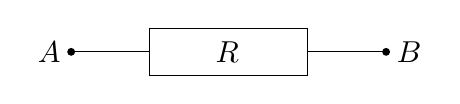
\begin{tikzpicture}
		\fill (0,0) circle(0.05);
		\draw (0,0)--(1,0);
		\draw (1,-0.3)rectangle(3,0.3);
		\node at(1.7,0)[right]{$R$};
		\draw (3,0)--(4,0);
		\fill (4,0) circle(0.05);
		\node at (0,0)[left]{$A$};
		\node at (4,0)[right]{$B$};
	\end{tikzpicture}
	\caption{一维的情况}
	\label{fig:1d}
\end{figure}
\par 二维的情况就是一个正方形,如图\ref{fig:2d}所示.我们也能很容易地算出来$AB$之间的等效电阻为$R$.
\begin{figure}[htbp]%二维情况
	\centering
	\begin{tikzpicture}
		\node at(0,0)[left]{$A$};
		\fill (0,0)circle(0.05);
		\foreach \x in{0,3}{
			\foreach \y in{0,4}{
				\draw (\x,\y)--(\x+1,\y);
				\draw (\y,\x)--(\y,\x+1);
			}
		} 
		\draw (1,-0.3)rectangle(3,0.3);
		\draw (1,3.7)rectangle(3,4.3);
		\draw (-0.3,1)rectangle(0.3,3);
		\draw (3.7,1)rectangle(4.3,3);
		\node at(1.7,0)[right]{$R$};
		\node at(1.7,4)[right]{$R$};
		\node at(-0.3,2)[right]{$R$};
		\node at(3.7,2)[right]{$R$};
		\fill (4,4)circle(0.05);
		\node at(4,4)[right]{$B$};
	\end{tikzpicture}
	\caption{二维的情况}
	\label{fig:2d}
\end{figure}
\par 下面我们来研究三维的情况.
\begin{figure}[H]%三维情况
	\centering
	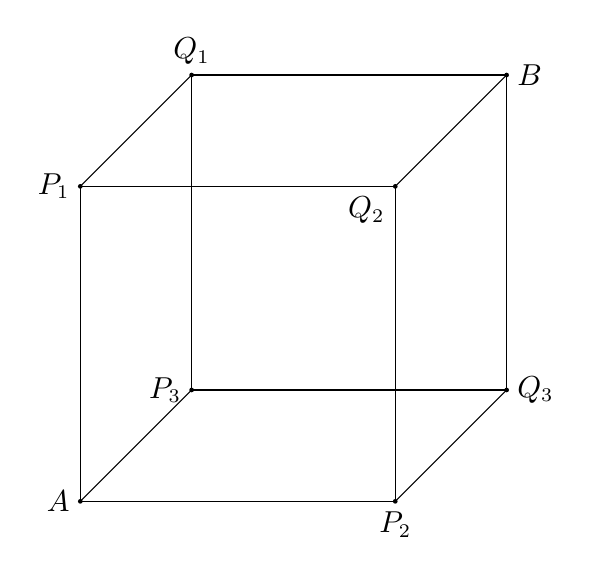
\begin{tikzpicture}
		\foreach \x in{0,4}{
			\foreach \y in{0,4}{
				\fill (\x,\y)circle(0.03);
				\fill (\x+1.414,\y+1.414)circle(0.03);
			}
		}
		\foreach \x in {0,4}{
			\draw (\x,0)--(\x,4);
			\draw (\x+1.414,1.414)--(\x+1.414,5.414);
			\draw (0,\x)--(4,\x);
			\draw (1.414,\x+1.414)--(5.414,\x+1.414);
		}
		\foreach \x in{0,4}{
			\foreach \y in{0,4}{
				\draw (\x,\y)--(\x+1.414,\y+1.414);
			}
		}
		\node at(0,0)[left]{$A$};
		\node at(5.414,5.414)[right]{$B$};
		\node at(0,4)[left]{$P_1$};
		\node at(4,0)[below]{$P_2$};
		\node at(1.414,1.414)[left]{$P_3$};
		\node at(1.414,5.414)[above]{$Q_1$};
		\node at(4,4)[anchor=north east]{$Q_2$};
		\node at(5.414,1.414)[right]{$Q_3$};
	\end{tikzpicture}
	\caption{三维的情况(图中未画出电阻)}
\end{figure}
\par 我们知道,图中的$P_1,P_2,P_3$是一组等势点,$Q_1,Q_2,Q_3$也是一组等势点.所以我们把电路化简为如图\ref{fig:3dsimple}所示结构.
\begin{figure}[htbp]%三维化简后的电路
	\centering
	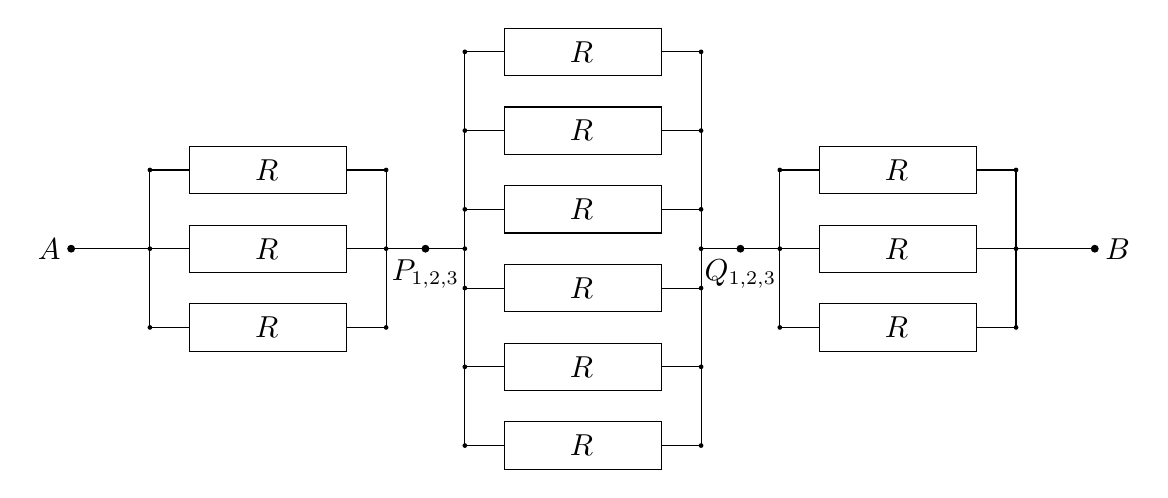
\begin{tikzpicture}
		\fill (0,0)node[left]{$A$} circle(0.05);
		\draw (0,0)--(1,0);
		\draw (1,-1)--(1,1);
		\foreach \x in{0,8}{
			\foreach \y in{-1,0,1}{
				\fill (1+\x,\y)circle(0.03);
				\draw (1+\x,\y)--(1.5+\x,\y);
				\draw (1.5+\x,\y-0.3)rectangle(3.5+\x,\y+0.3);
				\node at(2.2+\x,\y)[right]{$R$};
				\draw (3.5+\x,\y)--(4+\x,\y);
				\fill (4+\x,\y)circle(0.03);
			}
		}
		
		\draw (4,1)--(4,-1);
		\draw (4,0)--(5,0);
		\fill (4.5,0)node[below]{$P_{1,2,3}$} circle(0.05);
		\fill (5,0)circle(0.03);
		\draw (5,2.5)--(5,-2.5);
		\foreach \y in{2.5,1.5,0.5,-0.5,-1.5,-2.5}{
			\fill (5,\y)circle(0.03);
			\draw (5,\y)--(5.5,\y);
			\draw (5.5,\y-0.3)rectangle(7.5,\y+0.3);
			\node at (6.2,\y)[right]{$R$};
			\draw (7.5,\y)--(8,\y);
			\fill (8,\y)circle(0.03);
		}
		\draw (8,2.5)--(8,-2.5);
		\fill (8,0)circle(0.03);
		\draw (8,0)--(9,0);
		\fill (8.5,0)node[below]{$Q_{1,2,3}$} circle(0.05);
		\draw (9,1)--(9,-1);
		\draw (12,1)--(12,-1);
		\draw (12,0)--(13,0)node[right]{$B$};
		\fill (13,0)circle(0.05);
	\end{tikzpicture}
	\caption{三维情况的化简}
	\label{fig:3dsimple}
\end{figure}
\par 经过轻易的计算,得到$AB$之间的等效电阻为$\dfrac{R}{3} +\dfrac{R}{6}+\dfrac{R}{3}$,即$\dfrac{5}{6}R$.
\section{高维空间的代数表示}
显然,直观的几何无法描述高维空间,那么我们采用代数的方法解决.我们在$\mathbb{R}^n$中建立空间直角坐标系,坐标轴分别为$x_1,x_2,\cdots,x_n$.那么,我们可以列出在这个空间中的某一个正方体的所有顶点:$A_{(x_1,x_2,\cdots,x_n)}$,其中$x_i=0\text{或}1,i=1,2,\cdots,n$.那么与$A_{(x_1,x_2,\cdots,x_n)}$相邻的点有$n$个,分别为
\[A_{(1-x_1,x_2,\cdots,x_n)};\]
\[A_{(x_1,1-x_2,\cdots,x_n)};\]
\[\cdots\]
\[A_{(x_1,x_2,\cdots,1-x_n)}.\]
\par 对于一个点$A_{(x_1,x_2,\cdots,x_n)}$,与之相邻(即在一条棱上)的顶点可以通过将$x_1,x_2,\cdots,x_n$中的某一个1变为0,或将某一个0变为1得到.因此,将与点$A_{(x_1,x_2,\cdots,x_n)}$相连的所有棱所组成的集合记作 $E_{(x_1,x_2,\cdots,x_n)}$,即
\[E_{(x_1,\cdots,x_n)}=\{\left.\overline{A_{(x_1,x_2,\cdots,x_n)}A_t}\right|t=(x_1,\cdots,1-x_i,\cdots,x_n),i=1,2,\cdots,n\}.\]
将所有的顶点所组成的集合记作$V$,即
\[V=\{\left.A_{(x_1,x_2,\cdots,x_n)}\right|x_i=0\text{或}1,i=1,2,\cdots,n\}.\]
将所有的棱所组成的集合记作$E$,即
\[E=\bigcup\limits_{A\in V}E_A.\]
\section{问题解决}
设在$\mathbb{R}^n$中有一个立方体,其一组对顶点为$A_{(0,0,\cdots,0)}$与$A_{(1,1,\cdots,1)}$,每一条棱上都有一个电阻,其阻值为$R$.下面,求$A_{(0,\cdots,0)}$与$A_{(1,1,\cdots,1)}$之间的等效电阻.
\par 首先我们将点分为如下$(n+1)$类:
\[S_k=\left\{A_{(x_1,x_2,\cdots,x_n)}\left|\sum\limits_{i=1}^nx_i=k\right.\right\},k=0,1,\cdots,n.\]
\par 不难证明,$\left|S_k\right|=\mathrm{C}_n^k$.容易发现,对于每一个$S_i(i=0,1,\cdots,n)$,其中的每一个点都是等势点.那么我们可以将每一个$S_i$中的点都用导线连接在一起.这样,整个电路就变成了如图\ref{fig:simpler}所示的简单结构:
\begin{figure}[h]
	\centering
	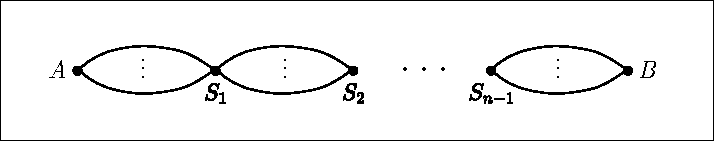
\includegraphics{Figure4.pdf}
	\caption{化简后的电路}
	\label{fig:simpler}
\end{figure}
\par 现在,问题的关键就是求出每一个$S_k$与$S_{k+1}(k=0,1,\cdots,n-1)$之间各有多少条 棱.我们将$S_k$与$S_{k+1}(k=0,1,\cdots,n-1)$之间的所有棱记作$E_k$,即
\[E_k=\left\{\left.\overline{A_1A_2}\right|A_1\in S_k,A_2\in S_{k+1}\right\}\cap E,k=0,1,\cdots,n-1.\]
现在我们来求$\left|E_k\right|$.
\par 注意到$E_k$中的每一条棱的顶点都分别是$S_k$与$S_{k+1}$中的点.而对于每一个 $A_{(x_1,x_2,\cdots,x_n)}\in S_k$,在$E_k$中与此点相连的棱为
\[E_{(x_1,x_2,\cdots,x_n)}\cap E_k,\]
即
\[\left\{\left. A_{(x_1,\cdots,x_i+1,\cdots,x_n)}\right|x_i=0\right\}.\]
\par 这个集合的元素个数为$x_1,x_2,\cdots,x_n$中0的个数,而$A_{(x_1,x_2,\cdots, x_n)}\in S_k$,所以$\sum\limits_{i=1}^nx_i=k$,所以0的个数为$n-k$.
\par 所以,我们有以下结论:
\[|E_k|=|S_k|\cdot(n-k)=\mathrm{C}_n^k\cdot(n-k).\]
\par   那么我们就可以计算$S_k$与$S_{k+1}$之间的电阻.由\ref{sec:chuanbing}:电阻的串并联中的(\ref{equ:binglian2})式,我们得到 $S_k$与$S_{k+1}$之间的电阻为
\[\frac{R}{\mathrm{C}_n^k\cdot(n-k)},\]
即
\[\frac{R\cdot k!(n-k)!}{n!(n-k)}.\]
再由(\ref{equ:chuanlian})式,我们得到$A_{(0,\cdots,0)}$与$A_{(1,1,\cdots,1)}$之间的等效电阻为
\[\sum\limits_{k=0}^{n-1}\frac{R}{\mathrm{C}_n^k\cdot(n-k)},\]
即
\[\sum\limits_{k=0}^{n-1}\frac{R\cdot k!(n-k)!}{n!(n-k)}.\]


\newpage
\hspace*{-2em}{\Large \textbf{参考文献}}\\
\begin{table}[htbp]%参考文献
	\centering
	\begin{tabular}{c|l}
		\toprule[1pt]
		{\small [1]}&{\small 刘炳昇,李容.物理(九年级上册)[M].南京:江苏凤凰科学技术出版社,2013.10.}\\
		{\small [2]}&{\small 黄东坡.精英物理大视野(九年级)[M].武汉:湖北人民出版社,2014.}\\
		\bottomrule[1pt]
	\end{tabular}
\end{table}

\end{document}